\documentclass[master,final,12pt]{iscs-thesis}

\etitle{Simple Solutions of Acyclic Horn Clauses for Program Verification}
\eauthor{Yuto Takei}
\esupervisor{Naoki Kobayashi}

\jtitle{�ץ�����ม�ڤΤ������۴� Horn �ὼ­����ˤ����뾮���ʲ������}
\jauthor{�ݰ� ͪ��}
\jsupervisor{���� ľ��}

\supervisortitle{Professor}
\date{August 28, 2013}

\usepackage{alltt}
\usepackage{amsmath}
\usepackage{amssymb}
\usepackage{algorithm}
\usepackage{algorithmic}
\usepackage[dvipdfmx]{graphicx}
\usepackage{listings}
\usepackage{multirow}
\usepackage{stmaryrd}
\usepackage{syntax}
\usepackage{url}
\usepackage{wrapfig}

\newcommand{\sembrack}[1]{[\![#1]\!}
\newcommand{\edge}[2]{#1\rightarrow#2}
\newcommand{\edgel}[3]{#1\xrightarrow{#2}#3}

\begin{document}

\begin{eabstract}
Automated theorem proving plays a crucial role in modern program
verification techniques.  In particular, in the context of software
model checking, the interpolation problem and its generalization
called \emph{Horn clause solving} have attracted special attention.
The latter problem asks for a solution for a set of acyclic Horn
clauses containing unknown predicate variables.  The solution, i.e., a
substitution for predicate variables, then serves as a candidate of
program invariants.  However, existing methods are unsatisfactory in
that they tend to generate too specific a solution, which does not
correspond to program invariants.

To address the problem above, we propose a new algorithm for solving
Horn clauses consisting of linear arithmetics and unknown predicate
variables.  The new algorithm tries to find small predicates, based on
the hypothesis that program's invariants tend to be simple formulas.
To this end, our algorithm prepares a template of linear arithmetic
formulas of a fixed size as a candidate of each unknown predicate, so
that Horn clause solving is reduced to linear programming.  The
algorithm iteratively increases the size of the templates until a
solution is found.  It enables us to construct relatively small
solutions in a reasonable time compared to existing algorithms.  We
have implemented and incorporated our Horn clause solver into MoCHi, a
software model checker for functional programs.  We have evaluated the
effectiveness of our approach through experiments.
\end{eabstract}

\begin{jabstract}
��ǯ�Υץ�����ม�ڵ��Ѥˤ����Ƥϡ���ư�������������פ�����ô�äƤ��롣�ä˥��եȥ����� ��ǥ븡����ʬ��Ǥϡ�������ꤪ��Ӥ��ΰ��̲��Ǥ��� Horn �ὼ­���꤬���ܤ򽸤�Ƥ�������Ԥ�����ϡ��۴Ĥ�����¸�ط�������ʤ���̤�ΤνҸ��ѿ���ʣ���ޤ� Horn ��ν���β���������Ǥ��롣Horn �ὼ­����β򡢤��ʤ�� Horn �ὸ��򹱿��Ȥ���褦�ʽҸ��ѿ��ؤ������ϡ��ץ����������Ѽ��θ���Ȥ����Ѥ����롣�������ʤ��顢Horn �ὼ­����δ�¸��ˡ�����Ϥ�����ʣ�������ü줹�������Ѽ��ˤʤ�ʤ����Ȥ�¿����
��Ҥ�������褹�뤿��ˡ����������������� Horn �ὼ­�����򤯿��������르�ꥺ�����Ƥ��롣�����Υ��르�ꥺ��ϡ��ץ���������Ѽ���ñ��ʼ���ɽ�����Ȥ�������Τ�Ȥǡ������ʽҸ���������ߤ롣������Ū��ã�����뤿�ᡢ���Υ��르�ꥺ��Ϥ����礭���������������ο�����̤�ΤνҸ��ѿ����줾����Ф�����������Horn �ὼ­����������ײ�ˡ�˵��夵���롣�����ơ��򤬸��Ĥ���ޤǿ����γ���򷫤��֤���������Ƽ�ˡ�Ǥϡ�����Ū�ʻ���������Ū�����ʲ�������뤳�Ȥ��Ǥ��롣�����ϡ����Υ��르�ꥺ���������ؿ�����������Υ��եȥ����� ��ǥ븡���� \textsc{MoCHi} ���Ȥ߹�������¸��ˤ�ꡢ��Ƽ�ˡ�ˤĤ��ư����ͭ�������ǧ������
\end{jabstract}

\maketitle

\begin{acknowledge}
Thank you.
\end{acknowledge}


\frontmatter
\tableofcontents

\mainmatter

\chapter{Introduction}

Automated theorem proving plays an important role in the modern
program verification.  Particularly in the context of verification
with model checking techniques, an automated theorem prover is used to
abstract a program with infinite states into a finite model so that a
model checker can virtually explore all possible program execution
paths.

One of the most common methods of such abstraction is predicate
abstraction\cite{conf/cav/GrafS97} within CounterExample-Guided
Abstraction Refinement (CEGAR) framework
\cite{conf/cav/ClarkeGJLV00,conf/popl/BallR02,conf/popl/HenzingerJMS02}.
An automated theorem prover finds appropriate predicates for every
program location.  Execution states at those locations are expressed
by a Boolean valuation of the given predicates.  If the abstraction is
too coarse and a model checker discovers an infeasible error execution
path, also called a spurious counterexample, the prover computes an
additional predicate at those program locations to refine the
abstraction.

In order to obtain an additional abstraction predicate at certain
program location along the infeasible path, one class of automated
theorem provers, called an interpolating theorem prover
\cite{journals/tcs/McMillan05,conf/vmcai/RybalchenkoS07}, computes a
logical separation between two sets of formula; the one consists of
constraints from the program entry point to the location, and the
other consists of the constraints from the location to the program
failure.  Those formulas are built from variable assignments and
assertions to be satisfied originated from conditional branches.

The computed logical separator is satisfied at the location under the
execution in the program along the discovered path, and any execution
paths which satisfies the predicate does not lead to the failure
state.  After the refinement, the counterexample is ruled out and the
same infeasible path is no longer found by the model checker.

However, existing interpolating theorem provers may return too complex
a solution which is heavily affected by the constraints of the
specific path.  It is not favorable in terms of the program
verification because a complex predicate may not be sufficient to rule
out resembling spurious paths in programs.  This causes the
verification process not to terminate because the model checker
infinitely discovers infeasible paths which pass the same program
location by loops or recursion calls on the different number of
iterations.

Ideally it is desired to discover an invariant formula for the
predicate abstraction.  We put a hypothesis that program invariants
tend to be simple formulas, and we propose a new interpolating
algorithm based on the hypothesis.  The algorithm tries to minimize
the number of conjunctions and disjunctions in a solution.  The
predicate obtained by this algorithm may become similar to the
invariant. We expect the number of iterations for model checking to
decrease as a result.

We also focus on solving constraint satisfaction problems over Horn
clauses with unknown predicate variables.  As well as interpolation,
Horn clause solving is another technique often used in program
verification for capturing program behaviors.  By computing the
solution for Horn clause problems, we obtain predicates that are true
at specific program locations along specific paths.  Furthermore it
may be possible to obtain predicates which are highly likely to be
program invariants by computing same predicates inside loops and
recursion calls on different iterations, or at the same location over
multiple paths.  By the previous hypothesis, we propose a Horn clause
solving algorithm which constructs as simple a solution as possible.

To confirm the effectiveness, we incorporated our algorithm into
existing software model checker \textsc{MoCHi}
\cite{conf/pldi/KobayashiSU11}.  We replaced the conventional Horn
clause solvers with our algorithms and tested some example programs to
verify the performance.  As a result, our algorithm was able to
compute a simple solution for most Horn clause solving problems.
Although we observed some test cases have experienced deterioration in
the number of verification cycles, there are some cases that are newly
verified by \textsc{MoCHi}.  Additionally, our algorithm improved a
performance in more than 70 percent of problems and achieved faster
computation than conventional method.  Eventually we have verified
certain effectiveness of our approach.

The rest of this thesis is structured as follows.
Chapter~\ref{chap:interpolation} shows detailed usage of interpolation
problems in program verification and proposes a new interpolating
algorithm to obtain simple solutions.  Chapter~\ref{chap:horn}
describes a Horn clause solving algorithm by extending the previous
interpolating algorithm.  Chapter~\ref{chap:experiment} describes
experiments and illustrates the result to confirm the effect of our
algorithms.  Chapter~\ref{chap:future} gives a discussion on further
possibilities for improvements. Chapter~\ref{chap:related} mentions
related work done by others.  Finally, Chapter~\ref{chap:conclusion}
reviews the impact of our research and brings the conclusion.

\chapter{Interpolation}
\label{chap:interpolation}

Among various program verification techniques, the interpolation has
been used to extract a program behavior as a logical formula.
Especially when one adopts software model checking technique with
predicate abstraction, the interpolation computes the abstraction
predicate along a spurious counterexample that a model checker
discovered.

It is done by computing a logical separation between the strongest
postcondition at the location and the weakest precondition to the
failure point at every program location.

However, by the existing interpolating theorem prover, we may not be
able to obtain a simple solution.  Consider the example below.
\begin{align*}
\varphi_1 : (x = 0 \wedge y = 0) \vee (x = 1 \wedge y = 1) \\
\varphi_2 : (x \neq 0 \wedge y = 0) \vee (x \neq 1 \wedge y = 1)
\end{align*}
Although one may be able to obtain $x = y$ as the simplest
interpolation between $\varphi_1$ and $\varphi_2$,
CSIsat\cite{conf/cav/BeyerZM08} returns
\begin{align*}
& ((((y \leq 0 \wedge -y \leq 0) \vee 1 = x) \wedge 1 \neq x) \vee ((1 \neq x \vee -y \leq -1) \wedge 1 = x) \vee 0 \neq x) \wedge \\
& \qquad (((0 \neq x \vee y \leq 1) \wedge (0 = x \vee y \leq 1)) \vee 1 \neq x) \wedge \\
& \qquad (((1 \neq x \vee -y \leq -1) \wedge 1 = x) \vee 0 = x) \wedge \\
& \qquad ((1 \neq x \wedge 1 = x) \vee (y \leq 0 \wedge -y \leq 0) \vee 0 \neq x) \wedge \\
& \qquad (1 = x \vee y \leq 0)
\end{align*}
as a solution.

We propose an interpolation algorithm which returns as simple a
solution as possible in terms of the number of conjunctions and
disjunctions.  Our algorithm focuses on interpolating problems on
linear arithmetic and it works in a constructive manner.


\section{Example}

Consider the following interpolation problem.

\begin{align*}
\frac
{A: (x \leq a) \wedge (a + 1 \leq y)}
{B: (y \leq b) \wedge (b + 1 \leq x)}
\end{align*}

Here, the linear arithmetic formulas A and B are inconsistent.  The
interpolant I for this problem is $x-y+1 \leq 0$, which is implied by
$A$ and inconsistent with $B$.  The vocabulary of $I$ is $\left\lbrace
x,y \right\rbrace$ and is over $A$'s vocabulary $\left\lbrace x,y,a
\right\rbrace$ and $B$'s $\left\lbrace x,y,b \right\rbrace$.

In computing the interpolant, we make a linear constraint of a
interpolant by applying Farkas's lemma.  First, we assign weight
parameters to every expression in conjunction form.

\begin{align*}
\begin{array}{r r r r r r l}
\lambda_1 : & -a & & +x & & & \leq 0 \\
\lambda_2 : & a & & & -y & +1 & \leq 0 \\
\hline
\lambda_3 : & & -b & & +y & & \leq 0 \\
\lambda_4 : & & b & -x & & +1 & \leq 0
\end{array}
\end{align*}

Because all expressions induce inconsistent as a whole, the sum of
weighted expressions should satisfy the following constraint.

\begin{align*}
\begin{array}{r l l}
- \lambda_1 + \lambda_2 & = 0 \quad & (a) \\
- \lambda_3 + \lambda_4 & = 0 & (b) \\
  \lambda_1 - \lambda_4 & = 0 & (x) \\
- \lambda_2 + \lambda_3 & = 0 & (y) \\
  \lambda_2 + \lambda_4 & > 0 & (\text{constant}) \\
\lambda_1, \ldots, \lambda_4 & \geq 0 & (\text{non-negative weight})
\end{array}
\end{align*}

With the linear constraint among $\lambda_i$ above, the interpolant is
represented as follows by the sum of weighted expressions from the
first formula groups.
\[ (- \lambda_1 + \lambda_2) a + \lambda_1 x - \lambda_2 y + \lambda_2 \leq 0 \]
One of the model of the linear constraint is $\lambda_1 = \lambda_2 =
\lambda_3 = \lambda_4 = 1$, and we obtain $x-y+1 \leq 0$ as a
solution.

% TODO: Better to mention multiple interpolants possible for one
% interpolating problem?


\section{Preliminaries}

Our algorithm aims to compute a Craig interpolant over linear
arithmetic formulas.


\paragraph{Craig Interpolation}
Given two logical formulas $A$ and $B$ that are inconsistent each
other, we call a new preposition $I$ a \emph{Craig interpolant}
\cite{journals/jsyml/Craig57} between $A$ and $B$ such that $I$ is
implied by $A$ and inconsistent with $B$.  $I$'s vocabulary must be
only free variables that appears in both $A$ and $B$.  If $A \wedge B$
is unsatisfiable, an interpolant $I$ always exists.

Our algorithm handles a linear expression $e$ which is in a form:
\[ a_1 x_1 + \cdots + a_n x_n + b \leq 0 \]
This expression contains coefficient parameters $a_1, \ldots, a_n$ and
a constant parameter $b$.  We treat a special expressions $\top$ as $0
\leq 0$ and $\bot$ as $1 \leq 0$.  The algorithm input and output is a
formula $\psi$ that consists of conjunctions and/or disjunctions of
linear expressions.
\[ \psi = e | e \wedge e | e \vee e | \top | \bot \]

In the simple interpolation, the algorithm receives two formulas in
$\psi$ and returns an interpolant in $\psi$.  For the later extension
to handle a symmetric interpolation problem, the algorithm receives
multiple formulas in $\psi$ and returns intermediate interpolants in
$\psi$.  For computing those interpolants over linear arithmetics, we
use Farkas's Lemma.


\paragraph{Farkas's Lemma on linear inequalities}
Let a linear inequality $e_i$ be represented as
$a_{i,1} x_1 + \cdots + a_{i,m} x_m <= a_{i,0}$.  Assuming that
$e_1,\cdots,e_n$ implies $e_0$, there exists
$\lambda_1,\cdots,\lambda_n$ that satisfy
\[a_{0,j} = \sum_{i=1}^n \lambda_i * a_{i,j} \quad (j=0, \ldots,m)\]

For the special case of Farkas's Lemma, we can state that:

Let a linear inequality $e_i$ be represented as
$a_{i,1} x_1 + \cdots + a_{i,m} x_m <= a_{i,0}$.  Assuming that
$e_1,\cdots,e_n$ implies $\bot$, there exists
$\lambda_1,\cdots,\lambda_n$ that satisfy
\[0 = \sum_{i=1}^n \lambda_i a_{i,j} \quad (j=1, \ldots, m) \wedge
0 > \sum_{i=1}^n \lambda_i a_{i,0}\]

Our interpolating algorithm make use of the latter version of Farkas's
Lemma.


\section{Algorithm}

Our algorithm aims to construct a relatively small interpolant in a
reasonable computation time for any input.  It also aims to obtain a
common solution among multiple interpolating problems.  These goals
are set because the algorithm is designed to be used as a sub-routine
for solving Horn clause satisfying problems
that are made while discovering predicates for abstraction
during the program verification.  These advantages of our algorithm
make it possible to return a relatively small predicates for those
problems. To accomplish these aims, the algorithm preserves a set of
interpolants during the computation, and executes operations
over interpolant sets.


\paragraph{Interpolation between conjunctions}
We first present an interpolating algorithm between two conjunctive
sets of linear inequalities $A = \left\lbrace e_1,\ldots,e_m
\right\rbrace$ and $B = \left\lbrace e_{m+1},\ldots,e_{m+n}
\right\rbrace$, where $e_i$ takes a form $\mathbf{a}_i \mathbf{x} + b
\leq 0$.  We assume that conjunctions of $A$ and $B$ are inconsistent.
For later convenience, we call this interpolating problem $\left( A, B
\right)$.  Then there exists an interpolating linear expression
$e_\star$ which satisfies
\begin{align*}
\left\lbrace e_1,\ldots,e_m \right\rbrace & \vdash e_\star \\
e_\star \wedge \left\lbrace e_{m+1},\ldots,e_{m+n} \right\rbrace & \vdash \bot
\end{align*}
For convenience, we assume that any expression $e_i$ have variables
$x_1, \ldots, x_a$.

According to the Farkas's lemma, there exists a set of assignments to
$\lambda_i$ to conclude $\bot$ from a set of linear expressions $A
\cup B$, namely,
\begin{align*}
& \exists \lambda_1, \ldots, \lambda_m. \\
& \sum_{i=1}^{m+n} \lambda_i \mathbf{a}_i = 0\wedge \sum_{i=1}^{m+n} \lambda_i b_i > 0
\end{align*}

Then, a linear combination of $A$'s formula with a weight $\lambda_1,
\ldots, \lambda_m$ becomes an interpolant $I$ between $A$ and $B$.
Note that any assignments to $\lambda_i$ that satisfy the expressions
above will let an expression $I$ to be an interpolant.  Considering
this, it is possible to obtain different interpolants for an
interpolating problem by computing different assignments to
$\lambda_i$.

This enables the algorithm to preserve a set of interpolants by a
linear expression template $a_1 x_1 + \cdots + a_n x_n + b \leq 0$
with a constraint to describe a possible space of coefficient
parameters $a_i$ and the constant parameter $b$.

In practical, we may use linear programming solvers to obtain a model
for $\lambda_i$.  By assigning concrete values to them, we can obtain
a concrete interpolant.


\paragraph{Computing a common interpolant}
Next we consider a method to compute a common interpolant across two
different interpolating problems.  That is, when given two
interpolating problems $\left(A_1, B_1 \right)$ and $\left(A_2, B_2
\right)$, the problem is about to compute the common interpolant I,
which is an interpolant for the first problem and the second one at
the same time.

This problem is used when solving a following Horn clause solving
problem, for instance.
\[
\implies
% TODO
\]

To accomplish this, we simply need to compute the intersection of
interpolant sets.  Let us call the interpolant space for the problems
$\left(A_1, B_1 \right)$ and $\left(A_2, B_2 \right)$,
$\mathcal{I}_1$, and $\mathcal{I}_2$.  In the previous method, a set
of interpolants was represented by a parameterized linear expression.
\begin{align*}
\mathcal{I}_1 = \left\lbrace \mathbf{a}_1 \mathbf{x} \leq b_1 \mid
C_1 (\mathbf{a}_1, b_1 ) \right\rbrace \\
\mathcal{I}_2 = \left\lbrace \mathbf{a}_2 \mathbf{x} \leq b_2 \mid
C_2 (\mathbf{a}_2, b_2 ) \right\rbrace
\end{align*}
To compute the intersection between them, it is sufficient to choose
the same assignments of parameters and let them satisfy the both
constraints $C_1$ and $C_2$.
\[ \mathcal{I} = \left\lbrace \mathbf{a} \mathbf{x} \leq b \mid
C_1(\mathbf{a}, b) \wedge C_2(\mathbf{a}, b) \right\rbrace \]

However, if such an assignment of $\mathbf{a}$ and $b$ does not exist,
no common solution exists across two problems because $\mathcal{I} =
\emptyset$.

By applying this approach, it is also possible to compute a common
interpolant among more than three problems.


\paragraph{Interpolation between logical formulas}
We now extend the algorithm so that it can handle general logical
formulas over linear arithmetic including disjunctions of linear
expressions.  Here the algorithm takes two logical formulas over
linear expressions as a problem input.  For convenience, we assume
that they are represented in disjunctive normal form (DNF).  The
solution for this problem is the interpolant that is a logical formula
of linear expressions.

First, consider the case of an interpolation problem between $A_1 \vee
A_2$ and $B$.  When $(A_1 \vee A_2) \wedge B$ is inconsistent, $A_1
\wedge B$ is necessarily inconsistent.  Let $\mathcal{I}_1$ denote the
set of interpolants for $(A_1, B)$.  In the same manner, let
$\mathcal{I}_2$ denote the set of interpolants for $(A_2, B)$.  We may
naturally obtain an interpolant set by the intersection $\mathcal{I} =
\mathcal{I}_1 \cup \mathcal{I}_2$ as a solution for $(A_1 \vee A_2,
B)$.  When the algorithm computes $\mathcal{I}$ by the previous
method, and it is $\emptyset$, we need to build a less simple solution
by
\[ \mathcal{I}' = \left\lbrace \left( I_1 \vee I_2 \right) \mid
I_1 \in \mathcal{I}_1 \wedge I_2 \in \mathcal{I}_2 \right\rbrace \]
Any formulas in the set $\mathcal{I}'$ are the interpolant for $(A_1
\vee A_2, B)$ because
\begin{align*}
\forall I \in \mathcal{I}. & A_1 \vdash I \wedge A_2 \vdash I \wedge I \wedge B \vdash \bot \wedge \\
& FV(I) = FV(A_1) \cup FV(A_2) \cup FV(B)
\end{align*}

Second, consider the case of an interpolation problem between $A$ and
$B_1 \wedge B_2$.
% TODO:

By combining these two ways of interpolant construction, we may be
able to build a small solution for more general cases like $(A_1,
\ldots, A_n)$ and $(B_1, \ldots, B_n)$.  In order to obtain a small
solution, we need to wisely choose the order of combining an
interpolant set.

\paragraph{Symmetric Interpolation}
TODO

\chapter{Horn clause solving}
\label{chap:horn}

We propose a new algorithm for solving recursion-less Horn clauses to
generate a solution which is as simple as possible.  This enables us
to obtain appropriate predicates that are suitable for predicate
abstraction in the program verification techniques.

The construction of the algorithm roughly consists of two parts.
\begin{itemize}
\item \textbf{Iterative Constraint Generation} is a process to build a
  constraint to compute a solution.  It starts from generating the
  weakest constraint in the sense that the resulting solution would
  not be simple yet.  The process iteratively strengthens a constraint
  until the strongest one while preserving the constraint
  satisfiability.  The strongest constraint gives a simple solution.
\item \textbf{Problem Restructuring} is a process to restructure the
  problem to obtain a less simple solution, if the constraint become
  unsatisfiable during the iterative constraint generation.  This
  process considers the unsatisfiable core of the constraint, and
  wisely enlarges the solution size.
\end{itemize}

All predicate variables in an input problem are assigned simple
templates.  Those predicate templates are parameterized.  In the
iterative constraint generation process, algorithm builds a linear
constraint that parameters in templates must satisfy.  This is done in
a constructive manner, and constraints are built in the order of
implication dependency in Horn clauses.  That is, when an input
problem has a Horn clause that has a predicate variable $P$ on its
left-hand and $Q$ on its right-hand, a constraint to describe
parameters in $P$'s template are first build before those in $Q$'s
template.  When all parameters in the whole problem are described, the
built constraint is evaluated to obtain a model.  Its instantiation
becomes an appropriate solution for the input problem.

The novelty of our algorithm lies in the incremental constraint
refinement.  The algorithm tries to solve from the weakest constraint
that an input problem allows that does not give a simple solution, and
gradually strengthen the constraint until it reaches to the simplest
solution that the problem has.  When a constraint becomes
unsatisfiable during this step, the algorithm analyzes the
unsatisfiable core and transforms the problem to obtain a less simple
solution.

This construction of the algorithm enables us to compute a relatively
simpler solution compared to existing algorithms while preserving the
computation cost in a reasonable time.

\section{Example}

\paragraph {Tree interpolation}
First, consider the following example.

\begin{align*}
x \leq 1 & \implies A(x) \\
y \leq 2 & \implies B(y) \\
A(x) \wedge B(y) & \implies 3x+2y \leq 10
\end{align*}

In this example, we would like to compute linear arithmetic formulas
for the predicate variables $A$ and $B$.  They appear only once on
both left-hand and right-hand globally in the problem.

We try to obtain a simple solution that is expressed by linear
expression templates, whose coefficients and constants are
parameterized.  Assume that they have following predicate templates.

\begin{align*}
A(x) : c_1 x + c_2 \leq 0 \\
B(y) : c_3 y + c_4 \leq 0
\end{align*}

By naturally encoding the first Horn clause with Farkas's lemma, we
obtain a linear constraint
$\lambda_1 = c_1 \wedge - \lambda_1 \geq c_2 \wedge \lambda_1 \geq 0$.
Any assignment to $ c_1, c_2, \lambda_1 $ which satisfies this will
make $A(x)$ valid for the first clause.  In the same manner, we obtain
$\lambda_2 = c_3 \wedge - 2 \lambda_2 \geq c_4 \wedge \lambda_2 \geq 0$
from the second clause, and 
$c_1 = 3 \lambda_3 \wedge c_3 = 2 \lambda_3 \wedge c_2 + c_4 \geq -10 \lambda_3 \wedge \lambda_3 > 0$
from the third.

One of the models satisfying all the constraints above is
$( c_1, c_2, c_3, c_4, \lambda_1, \lambda_2, \lambda_3 ) = (3, -3, 2, -4, 3, 2, 1)$.
By assigning them to the template, we obtain the following solution.

\begin{align*}
A(x) : 3 x - 3 \leq 0 \\
B(y) : 2 y - 4 \leq 0
\end{align*}

\paragraph {DAG problem solving}
Second, we explain a case that some predicate variables appear
multiple times on left-hand side in different Horn clauses.

\begin{align*}
x \leq 1 & \implies A(x) \\
A(x) \wedge A(y) & \implies x+y \leq 2
\end{align*}

Assigning a template $A(x) : c_1 x + c_2 \leq 0$, we obtain the same
constraint for the first clause as the previous example.

\begin{align} \label{eq:constr1}
\lambda_1 = c_1 \wedge - \lambda_1 \geq c_2 \wedge \lambda_1 \geq 0
\end{align}

Since we have $A$'s appearance twice on the second clause, it is
possible for $A$ to have two expressions each of which is used for
$A(x)$ and $A(y)$.  Although we need to use the same template for
multiple occurrences in order to compute the simplest solution, it may
make the whole constraints unsatisfiable if the simplest solution does
not exist.

Therefore, we generate a weaker constraint for the second clause that
allows different expressions of $A$ for multiple occurrence.  If the
whole constraint is satisfiable in the case, we try to solve in a
stronger constraint to generate a simple solution.

In this specific case, it is virtually equivalent to solve the
following problem in a weaker constraint.

\begin{align*}
\text{Problem:} \\
x \leq 1 & \implies A_1(x) \\
x \leq 1 & \implies A_2(x) \\
A_1(x) \wedge A_2(y) & \implies x+y \leq 2 \\
\\
\text{Templates:} \\
A_1(x) \text{ : } & c_{1,1} x + c_{2,1} \leq 0 \\
A_2(x) \text{ : } & c_{1,2} x + c_{2,2} \leq 0 \\
A(x) \text{ : } & A_1(x) \wedge A_2(x) \\
\end{align*}

By duplicating the constraint~\ref{eq:constr1} of $A$ for newly
created $A_1$ and $A_2$, we obtain the whole constraint as follows.

\begin{align*}
& \lambda_{1,1} = c_{1,1} \wedge - \lambda_{1,1} \geq c_{2,1} \wedge \lambda_{1,1} \geq 0 \wedge \\
& \lambda_{1,2} = c_{1,2} \wedge - \lambda_{1,2} \geq c_{2,2} \wedge \lambda_{1,2} \geq 0 \wedge \\
& c_{1,1} = \lambda_2 \wedge c_{1,2} = \lambda_2 \wedge c_{2,1} + c_{2,2} \geq 2 \lambda_2 \wedge \lambda_2 > 0
\end{align*}

This constraint is satisfiable and one model is
\[ ( c_{1,1}, c_{1,2}, c_{2,1}, c_{2,2}, \lambda_{1,1}, \lambda_{1,2}, \lambda_2 ) =
( 1, -1, 1, -1, 1, 1, 1 ) \] and the solution then becomes
$A(x) : (x -1 \leq 0) \wedge (x -1 \leq 0)$.

Since the weak constraint is satisfiable, we now refine the constraint
to obtain the better solution.  That is, simply eliminate the
duplication to build the following constraint for the original
template.

\begin{align*}
& \lambda_1 = c_1 \wedge - \lambda_1 \geq c_2 \wedge \lambda_1 \geq 0 \wedge \\
& c_1 = \lambda_2 \wedge c_1 = \lambda_2 \wedge 2 c_2 \geq 2 \lambda_2 \wedge \lambda_2 > 0
\end{align*}

Solving this constraint simply gives us a solution
$A(x) : x -1 \leq 0$.

\paragraph {Disjunctive Horn clause solving}
Finally, we explain a case that an input set of Horn clauses contain
disjunctions on left-hand side.

\begin{align*}
x \leq 0 \wedge -x \leq 0 & \implies A(x) \\
x+1 \leq 0 \vee -x+1 \leq 0 & \implies B(x) \\
A(x) \wedge B(x) & \implies 1 \leq 0
\end{align*}

Same as the previous examples, templates for predicate variables are
prepared.

\begin{align*}
A(x) : c_1 x + c_2 \leq 0 \\ B(x) : c_3 x + c_4 \leq 0
\end{align*}

The constraints generated are follows.

\begin{align*}
& \lambda_1 - \lambda_2 = c_1 \wedge 0 \geq c_2 \wedge \lambda_1 \geq 0 \wedge \lambda_2 \geq 0 \wedge \\
& \lambda_3 = c_3 \wedge \lambda_3 \geq c_4 \wedge \lambda_3 \geq 0 \wedge \\
& - \lambda_4 = c_3 \wedge \lambda_4 \geq c_4 \wedge \lambda_4 \geq 0 \wedge \\
& c_1 + c_3 = 0 \wedge c_2 + c_4 > 0
\end{align*}

The constraints here become unsatisfiable, and one possible
unsatisfiable core is:

\begin{align*}
\lambda_3 & = c_3 \\
\lambda_3 & \geq c_4 \\
- \lambda_4 & = c_3 \\
\lambda_4 & \geq c_4 \\
c_2 + c_4 & > 0 \\
0 & \geq c_2
\end{align*}

Because the unsatisfiable core contains constraints originating from
the disjunctions to be expressed in a single term template, we can
determine which predicate to relax its template to allow an enlarged solution.

Now we slightly change the problem and the template.

\begin{align*}
\text{Problem:} \\
x \leq 0 \wedge -x \leq 0 & \implies A(x) \\
x+1 \leq 0 & \implies B_1(x) \\
-x+1 \leq 0 & \implies B_2(x) \\
A(x) \wedge B_1(x) & \implies 1 \leq 0 \\
A(x) \wedge B_2(x) & \implies 1 \leq 0 \\
\\
\text{Templates:} \\
A(x) \text{ : } & c_1 x + c_2 \leq 0 \\
B_i(x) \text{ : } & c_{3,i} x + c_{4,i} \leq 0 \quad (i \in \left\lbrace 1,2 \right\rbrace ) \\
B(x) \text{ : } & B_1(x) \vee B_2(x)
\end{align*}

When we construct the constraints, as same as previous, we again
obtain an unsatisfiable core:

\begin{align*}
\text{Constraint:} \\
& \lambda_1 - \lambda_2 = c_1 \wedge 0 \geq c_2 \wedge \lambda_1 \geq 0 \wedge \lambda_2 \geq 0 \wedge \\
& \lambda_3 = c_{3,1} \wedge \lambda_3 \geq c_{4,1} \wedge \lambda_3 \geq 0 \wedge \\
& \lambda_3 = c_{3,2} \wedge \lambda_3 \geq c_{4,2} \wedge \lambda_3 \geq 0 \wedge \\
& - \lambda_4 = c_{3,1} \wedge \lambda_4 \geq c_4 \wedge \lambda_4 \geq 0 \wedge \\
& - \lambda_4 = c_{3,2} \wedge \lambda_4 \geq c_{4,2} \wedge \lambda_4 \geq 0 \wedge \\
& c_1 + c_{3,1} = 0 \wedge c_2 + c_{4,1} > 0 \wedge \\
& c_1 + c_{3,2} = 0 \wedge c_2 + c_{4,2} > 0
\\
\text{Unsatisfiable core:} \\
0 \geq c_2 \\
\lambda_3 = c_{3,1} \\ \lambda_3 \geq c_{4,1} \\
- \lambda_4 = c_{3,2} \\
c_1 + c_{3,1} = 0 \\ c_2 + c_{4,1} > 0 \\
c_1 + c_{3,2} = 0
\end{align*}

This time, the unsatisfiable core contains the constraints that
originate from


\begin{align*}
\text{Problem:} \\
x \leq 0 \wedge -x \leq 0 & \implies A_i(x) \quad (i \in \left\lbrace 1,2 \right\rbrace ) \\
x+1 \leq 0 & \implies B_1(x) \\
-x+1 \leq 0 & \implies B_2(x) \\
A_i(x) \wedge B_j(x) & \implies 1 \leq 0 \quad (i,j \in \left\lbrace 1,2 \right\rbrace ) \\
\\
\text{Templates:} \\
A_i(x) \text{ : } & c_{1,i} x + c_{2,i} \leq 0 \quad (i \in \left\lbrace 1,2 \right\rbrace ) \\
A(x) \text{ : } & A_1(x) \wedge A_2(x) \\
B_i(x) \text{ : } & c_{3,i} x + c_{4,i} \leq 0 \quad (i \in \left\lbrace 1,2 \right\rbrace ) \\
B(x) \text{ : } & B_1(x) \vee B_2(x)
\end{align*}

After this, we obtain the following constraint:

\begin{align*}
& \lambda_1 - \lambda_2 = c_{1,1} \wedge 0 \geq c_{2,1} \wedge \lambda_1 \geq 0 \wedge \lambda_2 \geq 0 \wedge \\
& \lambda_1 - \lambda_2 = c_{1,2} \wedge 0 \geq c_{2,2} \wedge \lambda_1 \geq 0 \wedge \lambda_2 \geq 0 \wedge \\
& \lambda_3 = c_{3,1} \wedge \lambda_3 \geq c_{4,1} \wedge \lambda_3 \geq 0 \wedge \\
& \lambda_3 = c_{3,2} \wedge \lambda_3 \geq c_{4,2} \wedge \lambda_3 \geq 0 \wedge \\
& - \lambda_4 = c_{3,1} \wedge \lambda_4 \geq c_4 \wedge \lambda_4 \geq 0 \wedge \\
& - \lambda_4 = c_{3,2} \wedge \lambda_4 \geq c_{4,2} \wedge \lambda_4 \geq 0 \wedge \\
& c_{1,1} + c_{1,2} + c_{3,1} = 0 \wedge c_{2,1} + c_{2,2} + c_{4,1} > 0 \wedge \\
& c_{1,1} + c_{1,2} + c_{3,2} = 0 \wedge c_{2,1} + c_{2,2} + c_{4,2} > 0
\end{align*}

By continuing this process, the process in the end generates a
predicate template that the solution will become.  Eventually, we
obtain the following solution.

\begin{align*}
A(x) \text{ : } & x \leq 0 \wedge -x \leq 0 \\
B(x) \text{ : } & x+1 \leq 0 \vee -x+1 \leq 0
\end{align*}

\section{Preliminaries}

For ease of discussion, our algorithm handles an input set of Horn
clauses by a \emph{Horn graph} that express the equivalent problem.
The graph is then used throughout the algorithm to represent the
problem.  A Horn graph is a labeled directed acyclic graph
$G=(V,E,\varphi)$.
\begin{itemize}
\item $V$ is a union of two disjoint sets of vertices; Horn term
  vertices $V_T$ and arrow vertices $V_\Rightarrow$.  Each vertex
  $u \in V_\Rightarrow$ has exactly one outgoing edge to some
  $v \in V_T$, denoted as $succ(u)$.
\item $E$ is a set of labeled edges, which are expressed in the form
  $(u,v,\theta)$ where $\theta$ is a finite map from variables to
  variables.
\item $\varphi: V_T \rightarrow L$ is a labeling function for Horn
  term vertices, where L is a set of elements of a predicate variable
  in the form $P(x_1, \ldots, x_{\mathrm{arity}(P)})$ or a linear
  inequality $a_1 x_1 + \cdots + a_n x_n + b \leq 0$.
\end{itemize}
There are two kinds of edges in a Horn graph;
\begin{itemize}
\item for $u \in V_T, v \in V_\Rightarrow$, an edge takes a form
  $(u,v,\theta)$, written $\edgel{u}{\theta}{v}$, or,
\item for $u \in V_\Rightarrow, v \in V_T$, an edge takes a form
  $(u,v,\emptyset)$, written $\edge{u}{v}$, where the mapping is
  empty.
\end{itemize}

We define the relation $\leadsto$ over $V_T$ as follows.
\[ u \mathop{\leadsto}^\theta v \Longleftrightarrow \exists a \in V_\Rightarrow;
\edgel{u}{\theta}{a} \wedge \edge{a}{v} \]
We may omit $\theta$ and write $u \leadsto v$ for convenience in later
discussions. By the assumption that $G$ is acyclic, both
$\rightarrow^+$ and $\leadsto^+$ are well-founded relations. $v_\bot$
is the greatest element with respect to both $\rightarrow^+$ and
$\leadsto^+$.

The meaning $\llbracket G \rrbracket $ of a Horn graph $G$ is a set of
Horn clauses $\mathcal{HC}_v$ for all vertices $v \in V_\Rightarrow$.
\begin{align*}
\mathcal{HC}_v & = \left( \bigwedge_{(u,v,\theta) \in E} \theta \varphi(u) \right) \Longrightarrow \varphi(succ(v)) \\
\llbracket G \rrbracket & = \bigwedge_{v \in V_\Rightarrow} \mathcal{HC}_v
\end{align*}
We implicitly assume each $\mathcal{HC}_v$ is universally quantified
by its all free variables $\textsc{FV}(\mathcal{HC}_v)$.

Horn term vertices with predicate variable labels are unique each
other that any of them do not have the same variable on their labels.
From now on, we may denote a Horn term vertex with a predicate
variable label by its predicate variable name if no ambiguity is
present.

Without loss of generality, we assume the existence of the
\emph{root vertex} $v_\bot \in V_T$ with linear expression labels
$1 \leq 0$, meaning $\bot$.  This is because if we have a Horn clause
$P \implies e$ which $e$ is a linear expression, we can convert it to
$P \wedge \neg e \implies 1 \leq 0$.  We also assume that other
vertices with linear expression labels have no incoming edges to them.

For simplicity of discussion, we define \emph{term arity} $k_v$ for
every Horn term vertex $v \in V_T$ with incoming edges.
\begin{align*}
k_v =
\begin{cases}
\mathrm{arity}(P) & \mbox{if } \varphi(v) = P(x_1,...,x_{\mathrm{arity}(P)}) \\
0 & \mbox{if } \varphi(v) = \bot
\end{cases}
\end{align*}
We let $K$ denote the maximum of $k_v$ over all $v \in V_T$.

A variable mapping label $\theta$ on edges is used to map the index of
one predicate variable to another.

The algorithm assigns a \emph{predicate template} for all predicate
variables in $G$. A \emph{predicate templateset} is a set of mappings
from a predicate variable to a predicate template.  A template for a
predicate variable $P(x_1, \ldots, x_n)$ is a formula $\psi$
constructed from the following definition.
\begin{align*}
\psi ::= & a_1 x_1 + \cdots + a_n x_n + b \leq 0 \mid \\
& \psi \wedge \psi \mid \psi \vee \psi
\end{align*}
A linear expression in the definition above may also be represented in
a equivalent vector form $\mathbf{a} \mathbf{x} + b \leq 0$ for short.
Parameters $\mathbf{a}$ and $b$ are specified by a linear constraint.

The solution of $G$ is a map $\rho$ from predicate variables to linear
predicates of the form $\lambda x_1, \ldots ,x_n. \psi$ where
parameters in $\psi$ are replaced with constant and $\rho[G]$ becomes
a tautology.  A solution is \textit{simple} if $\rho[P]$ is of the
form $\mathbf{a} \mathbf{x} + b \leq 0$ for every $P$ in
$\mathrm{dom}(\rho)$.

The problem of solving Horn clauses (represented by $G$) is to find a
solution of $G$ (and a simple solution if possible).

\section{Simple solution}

We first propose an algorithm to compute a simple solution for the
given Horn graph $G$ if one exists.  Later we add modifications to the
algorithm for the case that a simple solution does not exist for $G$.
In such a case, we transform the input graph $G$ to have a larger
solution template.

For each vertex $v \in V$, we define
$\Delta(v) = (\mathbf{a}_v \mathbf{x}_v + b_v \leq 0, C_v)$
, where
\begin{itemize}
\item $\mathbf{a}_v \mathbf{x}_v + b_v \leq 0$ is a linear inequality
  that contains coefficient variables $\mathbf{a}_v$ and a constant
  $b_v$, and
\item $C_v$ is a set of linear expressions on coefficient variables.
\end{itemize}
Intuitively, it denotes the set of inequalities:
\begin{align*}
\left\lbrace
 \mathbf{a}_v \mathbf{x}_v + b_v \leq 0 \mid
 \exists \left( \textsc{FV}(C_v)
  \setminus (\mathbf{a}_v \cup \left\lbrace b_v \right\rbrace
 \right); C_v
\right\rbrace
\end{align*}
For a predicate variable vertex,
$\mathbf{a}_v \mathbf{x}_v + b_v \leq 0$ serves as a predicate
template and $C_v$ describes the parameters $\mathbf{a}_v$ and $b_v$.

$C_v$ is defined by well-founded induction on $v$ with respect to the
relation $\rightarrow^+$. Then, $C_v$ can be shown as follows.
\begin{itemize}
\item For $v \in V_\Rightarrow$;
\begin{align*}
C_v & =
 \bigcup_{\edgel{u}{\theta}{v}} C_u \cup
 \bigcup_{0 < i \leq K}
 \left\lbrace
  \mathbf{a}_{v,i} = \sum_{\edgel{u}{\theta}{v}} \mathbf{a}_{u, \theta^{-1} (i)}
 \right\rbrace \\
 & \hspace{2cm} \cup
 \left\lbrace
  b_v \leq \sum_{\edgel{u}{\theta}{v}} b_u
 \right\rbrace \cup
 \bigcup_{k_{succ(v)} < i \leq K}
 \left\lbrace \mathbf{a}_{v,i} = 0 \right\rbrace
\end{align*}
\item For $v \in V_T$ such that
  $v \neq v_{\bot} \wedge \varphi(v) = \mathbf{a}_0 \mathbf{x}_v \leq b_0$
  where $\mathbf{a}_0$ and $b_0$ are constants;
\begin{align*}
C_v =
\left\lbrace
 \lambda_v \geq 0, \mathbf{a}_v = \lambda_v \mathbf{a}_0,
 b_v = \lambda_v b_0
\right\rbrace
\end{align*}
\item For $v \in V_T$ such that $\varphi(v) = P(\mathbf{x}_v)$;
\begin{align*}
C_v = & \bigcup_{\edge{u}{v}} \left( C_{u} \cup
\left\lbrace \mathbf{a}_u = \mathbf{a}_v, b_u = b_v \right\rbrace
\right)
\end{align*}
\item For $v_\bot$;
\begin{align*}
C_{v_\bot} = \bigcup_{\edge{u}{v_\bot}} \left( C_{u} \cup
\left\lbrace \mathbf{a}_u = \mathbf{0}, b_u > 0 \right\rbrace \right)
\end{align*}
\end{itemize}

Any model $\sigma$ to the constraint $C_{v_\bot}$ gives a simple
solution for $G$ if $C_{v_\bot}$ is satisfiable, i.e., we should have:

\begin{quote}
If $\models \sigma(C_{v_\bot})$, then $\rho$ defined by
\begin{align*}
 \rho = \left\lbrace
  \left( P, \sigma(\mathbf{a}_v \mathbf{x}_v \leq b_v) \right) \mid
  \forall v \in V_T; \varphi(v) = P(\mathbf{x}_v)
 \right\rbrace
\end{align*}
is a solution of $G$.
\end{quote}

If $C_{v_\bot}$ is unsatisfiable, no simple solution exists for $G$.
There are two cases that a simple solution does not exist for a
predicate variable.
\begin{itemize}
\item A predicate variable appears multiple times on left-hand of Horn
  clauses, and those appearances require different expressions as an
  assumption.
\item A predicate variable is implied by a disjunctive Horn clause,
  which has disjunctions on its left-hand, and a common premise that
  the disjunctions induce is not strong enough for solving a problem.
\end{itemize}

The first case occurs in a case like follows.
\begin{align*}
% conj.txt ... originated from uc/01.txt
\left( x \leq 0 \right) \wedge \left( y \leq 0 \right) & \implies P(x,y) \\
P(x,a) \wedge P(b,y) & \implies x+y \leq 0
\end{align*}
In this example, the predicate variable $P$ appears twice on the
second clause and they require different premises; $x \leq 0$ for the
first and $y \leq 0$ for the second.  They cannot be represented by
$\mathbf{ax} + b \leq 0$ template at the same time.

The second case occurs in a case like follows.
\begin{align*}
% disj-simp.txt ... originated from 23simp_neg.txt
\left( x+1 \leq 0 \right) \vee \left( -x+1 \leq 0 \right) & \implies P(x) \\
P(x,y) \wedge \left( x \leq 0 \right) \wedge \left( -x \leq 0 \right) & \implies \bot
\end{align*}
In this example, the predicate variable $P$ is implied by the first
clause, which is a disjunctive Horn clause.  As a simple solution, $P$
can take a common consequence that both of $x+1 \leq 0$ and
$-x+1 \leq 0$ induce.  However, such a simple linear expression does
not exist except for $0 \leq 0$, which is equivalent to $\top$, and it
is not sufficient to satisfy the second clause.

Both cases can be fixed by enlarging the solution template.


\section {Graph transformation}

If a simple solution does not exist for $G$, we try to give a less
simpler solution by transforming $G$ and relaxing the constraint
$C_{v_\bot}$.  This transformation takes place by considering the
unsatisfiable core $\mathcal{U}$.  An unsatisfiable core $\mathcal{U}$
is a subset of $C_{v_\bot}$ which is inconsistent itself.  Depending
on the reason for the absence of a simple solution, the way of the
transformation differs.

Algorithm~\ref{alg:solveHorn} shows the updated pseudo-code of our
Horn clause solving algorithm with the graph transformation.  It takes
an input Horn graph and returns a mapping between predicate variables
and linear arithmetic formulas.

\newcommand{\solveHorn}{\ensuremath{\mbox{\sc SolveHornGraph}}}
\newcommand{\genConstr}{\ensuremath{\mbox{\sc GenerateConstraint}}}
\newcommand{\transGraph}{\ensuremath{\mbox{\sc TransformGraph}}}

\begin{algorithm}
\caption{$ \solveHorn (G) $}\label{alg:solveHorn}
\begin{algorithmic}
\STATE {$v_\bot \gets $ the root node of $G$}
\STATE {$V_\star \gets \left\lbrace v_\bot \right\rbrace$}
\STATE {$T \gets $ initial predicate templateset for $G$}
\REPEAT
  \STATE {$C_{v_\bot} \gets \genConstr (G, v_\bot, V_\star)$}
  \IF {$C_{v_\bot}$ is satisfiable}
    \STATE {$\sigma \gets $ one model of $C_{v_\bot}$}
    \STATE {$V_\star \gets V_\star \cup \left\lbrace u \in V_T \mid \forall v \in V_\star; u \leadsto v \right\rbrace$}
  \ELSE
    \STATE {$\mathcal{U} \gets $ unsatisfiable core for $C_{v_\bot}$}
    \STATE {$(G, T) \gets \transGraph (G, T, \mathcal{U})$}
    \STATE {$V_\star \gets \left\lbrace v_\bot \right\rbrace$}
  \ENDIF
\UNTIL {$V_\star = V_T$}
\RETURN {$\sigma \left( T \right)$}
\end{algorithmic}
\end{algorithm}
\transGraph~procedure determines the unsatisfiable core of the
constraint and transform the Horn graph $G$ and predicate templates.
As mentioned earlier, two ways of graph transformation exist.

\paragraph{Conjunction split}
For the first case previously mentioned, the unsatisfiable core
$\mathcal{U}$ contains coefficient constraint expressions with a
coefficient parameter of certain predicate variable.  If the predicate
variable $P$ is the cause of unsatisfiability, some constraint
expressions in the unsatisfiable core have a parameter $a_{P,i}$
and/or $b_P$ in the following way.
\begin{align*}
% TODO:
& \exists v_a, v_b \in V_T; v_P \leadsto v_a \wedge v_P \leadsto v_b \wedge \\
& \left( \exists i, j, k;
\left\lbrace \left( \mathbf{a}_{v_a,j} = \ldots + \mathbf{a}_{v_P,i} + \ldots \right),
\left( \mathbf{a}_{v_b,k} = \ldots + \mathbf{a}_{v_P,i} + \ldots \right)
\right\rbrace \subseteq \mathcal{U} \right)
\end{align*}

In such a case, the predicate variable $P$ in question is copied to
$P_1, \ldots, P_n$ so that the different appearances of $P$ on
left-hand of Horn clauses can take different premises.  The solution
template of $P$ becomes the conjunction of $P_1, \ldots, P_n$.

<fig...>

Here, the graph $G=(V,E,\varphi)$ will be transformed into
$G'=(V',E',\varphi')$ such that:
\begin{align*}
V' & = V \setminus \left\lbrace v_P \right\rbrace \cup
  \left\lbrace v_{P_i} \mid \emptyset \right\rbrace \\
E' & = E \\
\varphi' & = \varphi
\end{align*}

Note that after this duplication of the predicate vertex $P$, in order
to induce different linear expressions for $P_1, \ldots, P_n$, it may
be necessary for preceding predicate variable vertices in $G$ to be
duplicated in the same manner as $P$. It is because that different
derivation of $P$'s implication relation may be required to get
different consequences.

However, succeeding predicate vertices of $P$ in $G$ and other
vertices than predecessors are not affected because those implications
that have $P$ in their assumption can selectively choose the premise
that $P_1, \ldots, P_n$ leads.

Therefore, this graph transformation only affects the predecessors of
$P$.

\paragraph{Disjunction split}
For the second case, the unsatisfiable core $\mathcal{U}$ contains
coefficient constraints that unifies induced linear expressions from
each term in disjunctions to be the same expression.  Similarly as
previous, if the predicate variable $P$ is the cause of
unsatisfiability, some constraint expressions in the unsatisfiable
core have a parameter $a_{P,i}$ and/or $b_P$ in the following way.
\begin{align*}
% TODO:
& \exists v_a, v_b \in V_T; v_P \leadsto v_a \wedge v_P \leadsto v_b \wedge \\
& \left( \exists i, j, k;
\left\lbrace \left( \mathbf{a}_{v_a,j} = \ldots + \mathbf{a}_{v_P,i} + \ldots \right),
\left( \mathbf{a}_{v_b,k} = \ldots + \mathbf{a}_{v_P,i} + \ldots \right)
\right\rbrace \subseteq \mathcal{U} \right)
\end{align*}

In such a case, the predicate variable $P$ in question is separated to
$P_1, \ldots, P_n$ each of which is implied by a term, which was
originally a part of a disjunction to imply $P$.  This intuitively
enables us to avoid generating a common linear expression that
disjunctive terms induces, and to propagate each term's premises to
$P$'s successors instead.

<fig...>

Here, the graph $G=(V,E,\varphi)$ will be transformed into
$G'=(V',E',\varphi')$ such that:
\begin{align*}
V' & = V \setminus \left\lbrace v_P \right\rbrace \cup
  \left\lbrace v_{P_i} \mid \emptyset \right\rbrace \\
E' & = E \\
\varphi' & = \varphi
\end{align*}

After this duplication of the predicate vertex $P$, unlike the
conjunction split, a disjunction at succeeding predicate
variable vertices ($R$ in this case) is produced.
\begin{align*}
(P_1 \wedge Q) \vee (P_2 \wedge Q) \implies R
\end{align*}
Also, predicate variables that appeared with $P$ in the same
assumption ($Q$ in this case) needs to be duplicated by conjunction,
so as to obtain different premises that go along with $P_i$.
Therefore, the effect of disjunction split may reach to neighboring
predicate vertices.


Consider these two ways of transformation, we show a pseudo-code for
\linebreak \transGraph~procedure.  The procedure is given the graph
$G$, the predicate templateset $T$, and the unsatisfiable core
$\mathcal{U}$. It returns the transformed graph $G'$ and the new
templateset $T'$.

\begin{algorithm}
\caption{$ \transGraph (G, T, \mathcal{U}) $}\label{alg:transGraph}
\begin{algorithmic}
% TODO:
\RETURN {$\left( G', T' \right)$}
\end{algorithmic}
\end{algorithm}


\paragraph{Combinatorial explosion in disjunctions}
Virtually, if multiple disjunctions exists in an input set of Horn
clauses, a na\"{i}ve way of building a solution is solve all
combinations of choices out of every disjunction and concatenate each
expression with conjunctions and/or disjunctions appropriately.  This
may cause a combinatorial explosion.

Consider example below. $e_i$ represents some conjunctions of linear
expressions.
% TODO: Can't we replace e_i with actual expressions?
\begin{align*}
(e_1 \vee e_2) \implies P \\ (e_3 \vee e_4) \implies Q \\ P \wedge Q \implies \bot
\end{align*}
In this example, a na\"{i}ve algorithm may solve following four
problems separately.
\begin{itemize}
\item $e_1 \implies P_1 \qquad e_3 \implies Q_1 \qquad P_1 \wedge Q_1 \implies \bot$
\item $e_2 \implies P_2 \qquad e_3 \implies Q_2 \qquad P_2 \wedge Q_2 \implies \bot$
\item $e_1 \implies P_3 \qquad e_4 \implies Q_3 \qquad P_3 \wedge Q_3 \implies \bot$
\item $e_2 \implies P_4 \qquad e_4 \implies Q_4 \qquad P_4 \wedge Q_4 \implies \bot$
\end{itemize}
Then the solution is built by follows.
\begin{itemize}
\item $P = ( P_1 \vee P_2 ) \wedge ( P_3 \vee P_4 )$
\item $Q = ( P_1 \vee P_3 ) \wedge ( P_2 \vee P_4 )$
\end{itemize}
However, this method is not efficient.

\paragraph{Algorithm}
To avoid this, our algorithm lets a predicate variable $P$ which is
disjunctively implied on the Horn graph $G$ to have a linear
expression that is consequences of all terms in the disjunction.  This
prevents the possibility of choices for disjunctions to be propagated
to succeeding vertices. The simple linear expression is propagated
instead.

On the other hand, the algorithm allows a predicate variable $P$ that
appears on multiple implications or appears multiple times in a single
implication to take different linear expressions as a premise at
different appearances.  This is for the algorithm to determine the
cause of unsatisfiability efficiently.  It is done by copying a
predicate templates and its parameters' constraint with appropriate
renaming.

The algorithm first execute this duplication on all predicate
variables with multiple appearances.  It is the weakest constraint
that the algorithm makes for the certain $G$.  Then, the algorithm
gradually reduces the number of vertices that are duplicated by each
time testing the satisfiability of the constraint.  When the
constraint becomes unsatisfiable at the certain iteration, the
algorithm can determine a predicate vertex which has to be split in a
conjunctive template.  If all the predicate variable constraints are
no longer duplicated and the constraint is the strongest, any model
for such constraint gives a simple solution under the Horn graph $G$
and the templateset $T$.

Note that duplicating the constraint in a na\"{i}ve way may cause the
constraint to exponentially grow in size.  Our algorithm prevent it by
simplifying a predicate vertex's constraint $C_v$ by quantifier
elimination when $v$ is duplicated in generating linear constraint.
For a predicate variable vertex $v_P$, variables except for the
coefficient parameter $\mathbf{a}_P$ and the constant parameter $b_P$
are eliminated.  Due to the constraints generation process, the
simplified constraint is also linear and can be efficiently check the
satisfiability.

We finally show the modified version of pseudo-code for $\genConstr$
procedure.  It produces the constraint $C_v$ for a given vertex $v$,
considering constraint duplication and simplification.

\begin{algorithm}
\caption{$ \genConstr (G, v, V_\star) $}\label{alg:genConstr}
\begin{algorithmic}
\STATE {$C \gets \emptyset$}
\FORALL {$v_\Rightarrow \in preds_G(v)$}
  \FORALL {$v_p \in preds_G(v_\Rightarrow)$}
    \IF {$\varphi (v_p)$ is a predicate variable}
      \STATE {$C \gets C \cup \genConstr (G, v_p, visited)$}
    \ELSE
      \STATE { $id$ }
    \ENDIF
  \ENDFOR
\ENDFOR
\end{algorithmic}
\end{algorithm}

\chapter{Experiment}
\label{chap:experiment}

We have incorporated our algorithm to the software model checker for
higher-order programs \textsc{MoCHi} \cite{conf/pldi/KobayashiSU11}.  It is
specifically designed to verify the correctness of higher-order
programs written in a small subset of ML.  This verification tool
abstracts a given input program by inferring dependent types for
higher-order programs \cite{conf/ppdp/UnnoK09}.

We implemented our proposed algorithm into \textsc{MoCHi} by two steps.  First,
we replace an existing theorem prover with our interpolating theorem
prover as a sub-routine for solving Horn clauses in dependent typing.
We used a method to obtain a common small interpolant across different
interpolating problems, while reducing a Horn clause problem into
interpolation \cite{conf/ppdp/UnnoK09}.  Second, we completely
replaced MoCHi's Horn solving algorithm with our algorithm.

For simplicity of the implementation, we assume that the linear
inequalities in the integer space.  Because of this, our algorithm
lost the completeness.  By using Motzkin's transpose theorem
\cite{journals/networks/Rajan90}, it is possible to handle linear
inequalities in both $\mathbf{ax} + b \leq 0$ and $\mathbf{ax} + b <
0$.

While solving interpolating problems, our algorithm treated linear
equalities in the form $\mathbf{ax} + b = 0$ specially without
normalizing into a conjunction of linear equalities so that the
algorithm obtain a linear equality in a set of interpolants.  It is
because we observed some cases that require an equality relation
between two variables but not an inequality as an program invariant.

Note that, however, in Horn clauses solving problems, when a predicate
variable $P$ needs to take an equality $=$ or negation $\neq$, the
predicate template grows during the solving process as
$\mathbf{ax}-b \leq 0 \wedge -\mathbf{ax}+b \leq 0$ in the former
case, and $\mathbf{ax}-b+1 \leq 0 \vee -\mathbf{ax}+b+1 \leq 0$ in the
latter case.  We also thought it possible to obtain predicates that
are similar to program invariants by considering multiple paths.

For linear constraint satisfaction, we used GNU Linear Programming Kit
(GLPK) first for its light computation load.  For Horn clause solving
however, our implementation make use of Z3 \cite{conf/tacas/MouraB08}
as an SMT solver to obtain unsatisfiable core of the constraints.

\section{Interpolating theorem prover}

As an experiment of our interpolating algorithm, we compared the
quality of resulting interpolants with
ones that \textsc{CSIsat} \cite{conf/cav/BeyerZM08} generates.
It combines linear arithmetic reasoning and SAT-based logical reasoning.
\textsc{CSIsat} is mainly used as a sub procedure of current \textsc{MoCHi}.  Note that
it may return different interpolants for an interpolating problem
because of the randomized algorithm.  Results shown below
are ones that are randomly chosen.
\textsc{Yint} represents our interpolating algorithm.

\begin{itemize}
\item Disjunctive interpolation in $A$.
\[\begin{array}{r c}
\varphi_A : & (x-1 \geq 0) \vee (x+1 \leq 0) \\
\hline
\varphi_B : & x=0
\end{array}\]
The result for this:
\[\begin{array}{l c}
\text{\textsc{Yint}} & (x+1 \leq 0) \vee (-x+1 \leq 0) \\
\text{\textsc{CSIsat}} & (-x \leq -1 \vee x \leq -1)
\end{array}\]
\item Disjunctive interpolation in $B$.
\[\begin{array}{r c}
\varphi_A : & x=0 \\
\hline
\varphi_B : & (x-1 \geq 0) \vee (x+1 \leq 0)
\end{array}\]
\[\begin{array}{l c}
\text{\textsc{Yint}} & -x=0 \\
\text{\textsc{CSIsat}} & (-x \leq 0 \wedge x \leq 0)
\end{array}\]
\item Complex formula in $A$.
% complicated disj
\[\begin{array}{r c}
\varphi_A : & ((x-5<0) \wedge (-x<0)) \vee ((x<0) \wedge (-x-5<0)) \\
\hline
\varphi_B : & x=0
\end{array}\]
\[\begin{array}{l c}
\text{\textsc{Yint}} & (x+1 \leq 0) \vee (-x+1 \leq 0) \\
\text{\textsc{CSIsat}} & (x < 0 \vee -x < 0)
\end{array}\]
\end{itemize}
For those problems that are simple enough, \textsc{Yint} and \textsc{CSIsat} returns the
same results.

Next we tried the problem that an equality interpolant exists.
% equality
\[\begin{array}{r c}
\varphi_A : & x=0 \\
\hline
\varphi_B : & x-1=0
\end{array}\]
\[\begin{array}{l c}
\text{\textsc{Yint}} & x=0 \\
\text{\textsc{CSIsat}} & x \leq 0
\end{array}\]

\bigskip\centerline{}

% quantifier
\[\begin{array}{r c}
\varphi_A : & (y-z=0) \wedge (x-z=0) \\
\hline
\varphi_B : & (-w+y+1 \leq 0) \wedge (-w+x \geq 0)
\end{array}\]
\[\begin{array}{l c}
\text{\textsc{Yint}} & x-y=0 \\
\text{\textsc{CSIsat}} & x-y \leq 0
\end{array}\]
Because our algorithm handles linear equalities special, our algorithm
makes an effort to return an interpolant of linear equality if one
exists.

Additionally, as the follwing results of \textsc{Yint} shows, if a
simple interpolant exists for a given problem, our algorithm tries
such result.
\[\begin{array}{r c}
\varphi_A : & ((-y+1 \leq 0) \wedge (-x \leq 0)) \vee ((-y \leq 0) \wedge (-x+1 \leq 0)) \\
\hline
\varphi_B : & ((y+1<0) \wedge (x<0)) \vee ((y<0) \wedge (x+1<0))
\end{array}\]
\[\begin{array}{l c}
\text{\textsc{Yint}} & -x \leq 0 \\
\text{\textsc{CSIsat}} & (((x < 0 \vee -x \leq 0) \wedge 0 \leq x) \vee ((y < 0 \vee -y \leq 0) \wedge 0 \leq y))
\end{array}\]

\bigskip\centerline{}

\[\begin{array}{r c}
\varphi_A : & (x-1=0) \vee (x+1=0) \\
\hline
\varphi_B : & (x-2=0) \vee (x=0) \vee (x+2=0)
\end{array}\]
\[\begin{array}{l c}
\text{\textsc{Yint}} & (-x-1=0) \vee (-x+1=0) \\
\text{\textsc{CSIsat}} & ((-x \leq -1 \vee x \leq -1) \wedge (-x \leq 1 \vee - x \leq - 1) \wedge (x \leq - 1 \vee x \leq 1))
\end{array}\]

Finally, we showed some test cases that may occur in practical interpolation.

\[\begin{array}{r c}
\multirow{2}{*}{$\varphi_A$}
& ((x-y-1 \leq 0) \wedge (-x+y-2 \leq 0) \wedge (x+y-1 \leq 0) \wedge (-x-y-2 \leq 0)) \vee \\
& ((x-y-2 \leq 0) \wedge (-x+y-1 \leq 0) \wedge (x+y-2 \leq 0) \wedge (-x-y-1 \leq 0)) \\
\hline
\varphi_B : & (x=0 \wedge y=2) \vee (x=0 \wedge y=-2)
\end{array}\]
\[\begin{array}{l c}
\text{\textsc{Yint}} & (-x+17y-33 \leq 0) \wedge (x-17y-33 \leq 0) \\
\text{\textsc{CSIsat}} & ((-1 \leq (x + y) \vee (x + -y) \leq 1) \wedge (-1 \leq (x + -y) \vee (x + y) \leq 1))
\end{array}\]

\begin{figure}
\begin{center}
\includegraphics[scale=1]{figures/int1.eps}
\end{center}
\caption{Interpolation}
\end{figure}

\bigskip\centerline{}

\[\begin{array}{r c}
\multirow{2}{*}{$\varphi_A$}
& ((y+1=0) \wedge (x-1=0)) \vee ((y+1=0) \wedge (x+1=0)) \vee \\
& ((y-1=0) \wedge (x+1=0)) \vee ((y-1=0) \wedge (x-1=0)) \\
\hline
\multirow{2}{*}{$\varphi_B$}
& ((y+2 \leq 0) \wedge (x-2 \geq 0)) \vee ((y+2 \leq 0) \wedge (x+2 \leq 0)) \vee \\
& ((y-2 \geq 0) \wedge (x+2 \leq 0)) \vee ((y-2 \geq 0) \wedge (x-2 \geq 0))
\end{array}\]
\begin{tabular}{l c}
\textsc{Yint} & $(-2y-3 \leq 0) \wedge (2y-3 \leq 0)$
\end{tabular}

\begin{figure}
\begin{center}
\includegraphics[scale=1]{figures/int2.eps}
\quad
\includegraphics[scale=1]{figures/int3.eps}
\end{center}
\caption{Interpolation}
\end{figure}

\bigskip\centerline{}

\textsc{CSIsat}
\begin{align*}
& ((-y \leq 1 \wedge y \leq -1) \vee (-y \leq -1 \wedge x \leq 1) \vee x \leq -1) \wedge \\
& \qquad (-x \leq 1 \vee -x \leq -1 \vee -y \leq -1) \wedge \\
& \qquad (-x \leq 1 \vee -x \leq -1 \vee y \leq -1) \wedge \\
& \qquad (-x \leq -1 \vee x \leq -1)
\end{align*}

\[\begin{array}{r c}
\varphi_A & (x=1 \wedge y=1) \vee (x=0 \wedge y=0) \\
\hline
\varphi_B & (x=1 \wedge y \neq 1) \vee (x=0 \wedge y \neq 0)
\end{array}\]
\begin{tabular}{l c}
\textsc{Yint} & $x-y=0$
\end{tabular}

\textsc{CSIsat}
\begin{align*}
& ((((y \leq 0 \wedge -y \leq 0) \vee 1 = x) \wedge 1 \neq x) \vee ((1 \neq x \vee -y \leq -1) \wedge 1 = x) \vee 0 \neq x) \wedge \\
& \qquad (((0 \neq x \vee y \leq 1) \wedge (0 = x \vee y \leq 1)) \vee 1 \neq x) \wedge \\
& \qquad (((1 \neq x \vee -y \leq -1) \wedge 1 = x) \vee 0 = x) \wedge \\
& \qquad ((1 \neq x \wedge 1 = x) \vee (y \leq 0 \wedge -y \leq 0) \vee 0 \neq x) \wedge \\
& \qquad (1 = x \vee y \leq 0)
\end{align*}


\section{Horn clause solving}

As an Horn clause solver we incorporated our Horn clause solver to MoCHi.

\begin{figure}
\begin{center}
\includegraphics[scale=.6]{figures/unsat2.eps}
\quad
\includegraphics[scale=.6]{figures/unsat3.eps}
\end{center}
\caption{Result obtained from \textsc{MoCHi} with Horn clause solver \textsc{CSIsat} and
\textsc{Yhorn}}
\end{figure}

We obtained better result in some cases compared to the one we had in \textsc{CSIsat}.

%\begin{figure}
%\begin{center}
%\includegraphics[scale=.8]{figures/time.eps}
%\end{center}
%\caption{Time consumption ration of Yhorn compared to \textsc{CSIsat}}
%\end{figure}

However we take a longer time for solving the same Horn clauses, which
means further optimization is required for our algorithm.

\chapter{Related work}
\label{chap:related}

Interpolating theorem proving have played an important role in program
verification.  For instance, it is applied to invariant generation for
verification condition based program analysis, and predicate discovery
for the model checking by CEGAR with predicate abstraction.  The
former method is adopted when analyzing input programs by axiomatic
semantics such as Hoare logic, and synthesizing invariants from
strongest postconditions and weakest preconditions at various program
locations.  The latter one is used when model check a system with
infinite states by abstracting its data domain with predicates into a
finite system.

Interpolation in invariant generation is first proposed
by \cite{conf/cav/McMillan03} for unbounded model checking of a state
transition system, which does not specify the number of transition
steps to verify in iterative state exploration.  Instead of
constructing a Boolean Decision Diagram (BDD), this method adopted
Craig interpolation for compute the image fixedpoint for inductive
invariant generation.

Inspired from this method, \cite{conf/popl/HenzingerJMM04} adopted the
use of Craig interpolation for predicate discovery in CEGAR framework
with predicate abstraction, and proposed a method to derivate an
interpolant from counterexample's refutation proof derivation tree.
This work implemented the proposed method into the \textsc{Blast}
software model checker
\cite{conf/popl/HenzingerJMS02,journals/sttt/BeyerHJM07} and verified
the effectiveness of interpolants for predicate abstraction through an
experiment of C program verification.

\paragraph{Development of interpolating theorem provers}
An interpolating prover \textsc{FOCI} \cite{website/foci} was
developed under the comprehensive work on quantifier-free interpolant
generation over the theory of linear arithmetic and uninterpreted
function symbols (LI+UIF) theory \cite{journals/tcs/McMillan05}.  At
the same time, various applications of interpolants for model checking
was proposed \cite{conf/tacas/McMillan05}. They incorporated the
algorithm into \textsc{Z3} SMT solver \cite{conf/tacas/MouraB08} and
it is possible to generate an interpolant from proofs generated by
\textsc{Z3} \cite{conf/fmcad/McMillan11}.


On the other hand, an interpolating method without using proof
derivation was proposed that made use of the specific characteristics
of linear arithmetics.  \textsc{CLP-Prover} \cite{website/clp} is
another interpolating theorem prover with the theoretical ground of
linear constraint generation.  It focuses on interpolation over LI+UIF
and adopts Farkas's Lemma \cite{journals/networks/Rajan90} for give a
reasoning for handling linear
inequalities \cite{conf/vmcai/RybalchenkoS07, conf/cav/Rybalchenko10}.
Because the \textsc{CLP-Prover} cannot handle logical formulas with
disjunctions, we extended the basic principle of this work to handle
disjunctions. Our interpolating algorithm was strongly inspired.

Note that the suggested interpolating algorithms so far were not
complete in the sense that the algorithms may not be able to find a
suitable predicate that is necessary for a model checker to terminate.
Although it may be possible to simply enumerate interpolants in a
complete manner, its cost is not negligible with respect to the
computation time because of combinatorial explosion.
\cite{conf/tacas/JhalaM06} suggested a practical way to
obtain complete interpolating algorithm.

\paragraph{Extension to Horn clause solvers}
As a model checking technique, various methods are proposed to
efficiently eliminate spurious counterexamples from an abstract system
and terminate CEGAR process with less number of cycles.  Main
principles are support of disjunctive problems and extension to Horn
clause solvers.

One of them is work done by \cite{conf/pldi/BeyerHMR07} to eliminate
spurious paths that pass over loops.  The method converts a
counterexample from the model checker into a path that is a subgraph
of program's control flow graph, and performs a invariant synthesis
over it.  Here, the control flow graph may contain loops, it is not
sufficient by the conventional interpolation, and rather it required a
disjunctive reasoning.

As we explained in Chapter~\ref{chap:interpolation}, when
interpolating between two logical formulas, it is necessary to combine
interpolants by conjunctions and disjunctions.  To minimize the number
of terms efficiently, \cite{conf/cav/AlbarghouthiM13} suggested a
non-deterministic method of building such interpolant by wisely
sampling a half-interpolant.

For solving a complex system, it may not be possible to analyze
system's behavior by interpolation.  \cite{conf/aplas/GuptaPR11}
showed an algorithm to solve Horn clauses over LI+UIF.

One of the most important applications of Horn clause solving is
verifying higher-order functional programs.  Interpolation is used as
a sub procedure of solving Horn clauses for dependent type inference
\cite{conf/ppdp/UnnoK09, conf/pepm/SatoUK13} in this context. In
\textsc{MoCHi}, the refinement types are given for values and
variables for program abstraction.  Horn clause solving is necessary
for inferring the refinment types.  \cite{conf/popl/Terauchi10}
suggested a method for dependent type inference algorithm as well.

Another application of Horn clause solving is the verification of
concurrent systems \cite{conf/popl/GuptaPR11}. The work suggested to
describe a multi-thread program's behavior in Horn clauses and perform
model checking over abstract system.

Finally, some research integrated disjunctive interpolating methods
with Horn clause solving algorithms.  In previously suggested methods
in \cite{conf/popl/HenzingerJMM04, conf/cav/McMillan06}, it was not
possible to consider multiple spurious
paths.  \cite{conf/cav/RummerHK13} suggested an algorithm to solve
disjunctive Horn clauses, and it became possible to give a stronger
reasoning on a program invariant where multiple paths meet.  It also
enabled the abstraction for the case that branch conditions had a
disjunctive operator in them.

\paragraph{Recent work}

One of the recent extensions of Horn clause solving is to handle
non-linear constraints \cite{conf/cav/DaiXZ13}.  For instance, if a
program contains integer multiplication operation over variables,
existing algorithms cannot infer program invariants.  This research
aims to overcome the hurdle and infer non-linear invariants for
program verification.

As another direction of extension, some works are done for solving
Horn clauses with quantified consequences \cite{conf/sas/BjornerMR13,
conf/cav/BeyenePR13}.  They are used to abstract more complex systems
efficiently.

\chapter{Future Work}
\label{chap:future}

\paragraph{Non-linear extension}
\cite{conf/cav/DaiXZ13}

\chapter{Conclusion}
\label{chap:conclusion}

In this thesis, we have suggested new algorithms to discover
predicates that are suitable for program verification.  We put a
hypothesis that the program invariants are prone to be expressed in
simple expressions.  Based on this hypothesis, our algorithm tries to
obtain a small predicate with a fewer number of terms.

To accomplish this goal on Craig interpolation over linear
arithmetics, we first explained a method to reduce interpolation into
linear constraint generation by using Farkas's Lemma.  This method
preserves a set of solutions during the computation process so to make
it possible to choose a small solution later. This enabled a Horn
clause solver to build small solutions when it uses the method as a
subroutine due to the ability to choose a common predicate among
different interpolating problems. Additionally, we mentioned the
possibility of choosing small solutions in interpolating general
formulas by wisely choose the order to combine set of solutions during
the computation. In the end we extended the method to solve symmetric
interpolation problems to perform predicate discovery at multiple
locations in the program at the same time.

Next we extended our interpolating method to solve recursion-less
disjunctive Horn clauses.  Same as previous, this method also
describes a set of predicates for each predicate variable in linear
constraints.  The algorithm builds a solution in constructive manner
and is thus scalable for the size of input problems. If the algorithm
fails to find a simple solution, it tries to find a larger solution in
error-guided manner.  By observing an unsatisfiable core, the
algorithm enlarges a size of solution for certain predicates.  We have
also proposed to simplify linear constraints by quantifier elimination
for preventing exponential growth of them.

We have incorporated our algorithm into MoCHi and confirmed the
effectiveness to a certain level.

We would like to extend the algorithm further to achieve better
performance in constraint generation.  It is also desired to support
uninterpreted function symbols in our theory.


\bibliographystyle{plain}
\bibliography{./biblio}

\end{document}
